Per svolgere quest'esperienza è stato utilizzato il seguente apparato sperimentale:
\begin{itemize}
	\item Vaschetta trasparente di plastica di altezza $D$
	\item Asta di lunghezza $D_0>D$
	\item Metro a nastro
	\item Carta millimetrata
	\item Riga
	\item Nastro adesivo
	\item Morsa da tavolo per fissare l'asta 
\end{itemize}


\begin{table}[H]
	\centering
	\begin{tabular}{|c|c|}
		\hline
		\textbf{Strumenti di misura} & \textbf{Risoluzione} \\
		\hline
		Metro a nastro & $1\ mm$ \\
		Carta millimetrata & $1\ mm$ \\
		Riga & $1\ mm$ \\
		\hline
	\end{tabular}
	\caption{Risoluzione degli strumenti di misura utilizzati}
	\label{tab:}
\end{table}


\begin{figure}[H]
	\centering
	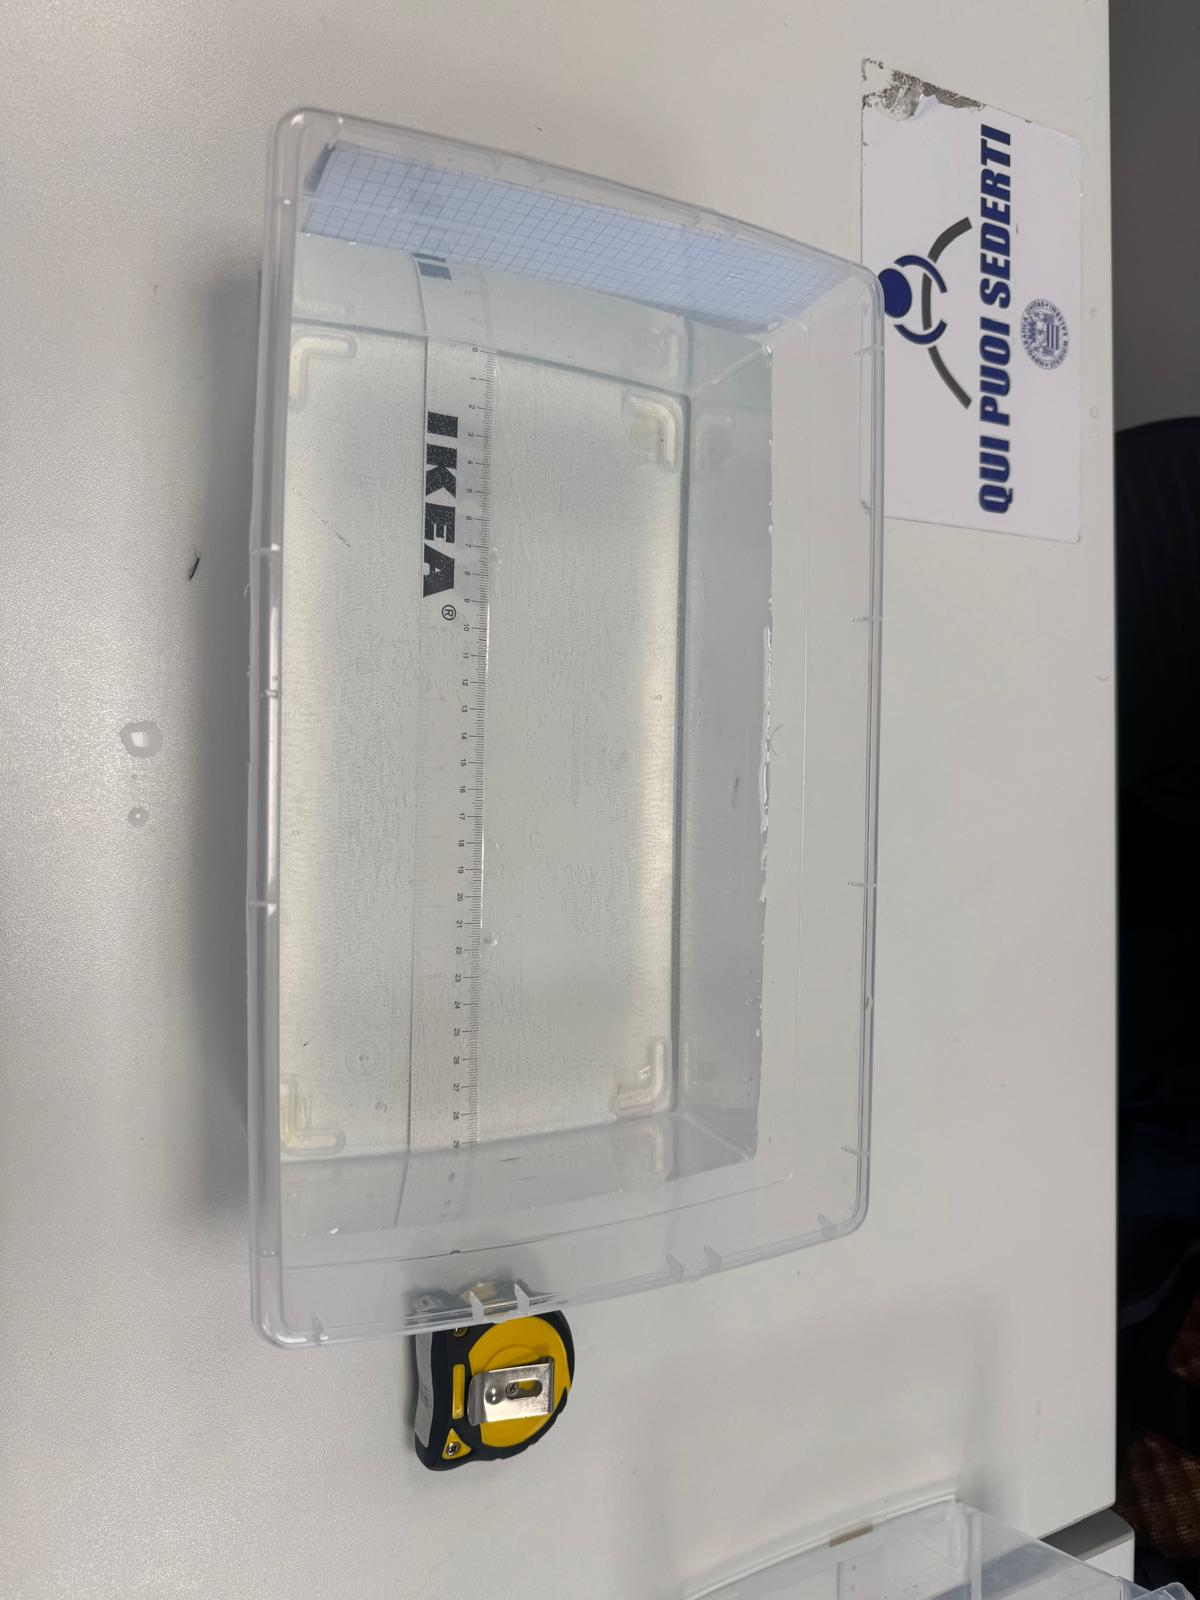
\includegraphics[width=0.65\textwidth]{./figures/vaschettaemetro}
	\caption{Vaschetta utilizzata per l'esperimento. Sulla sua base è posta la carta millimetrata per permettere la determinazione del punto $O'$. Alla sua destra è presente il metro a nastro utilizzato.}
\end{figure}

\begin{figure}[H]
	\centering
	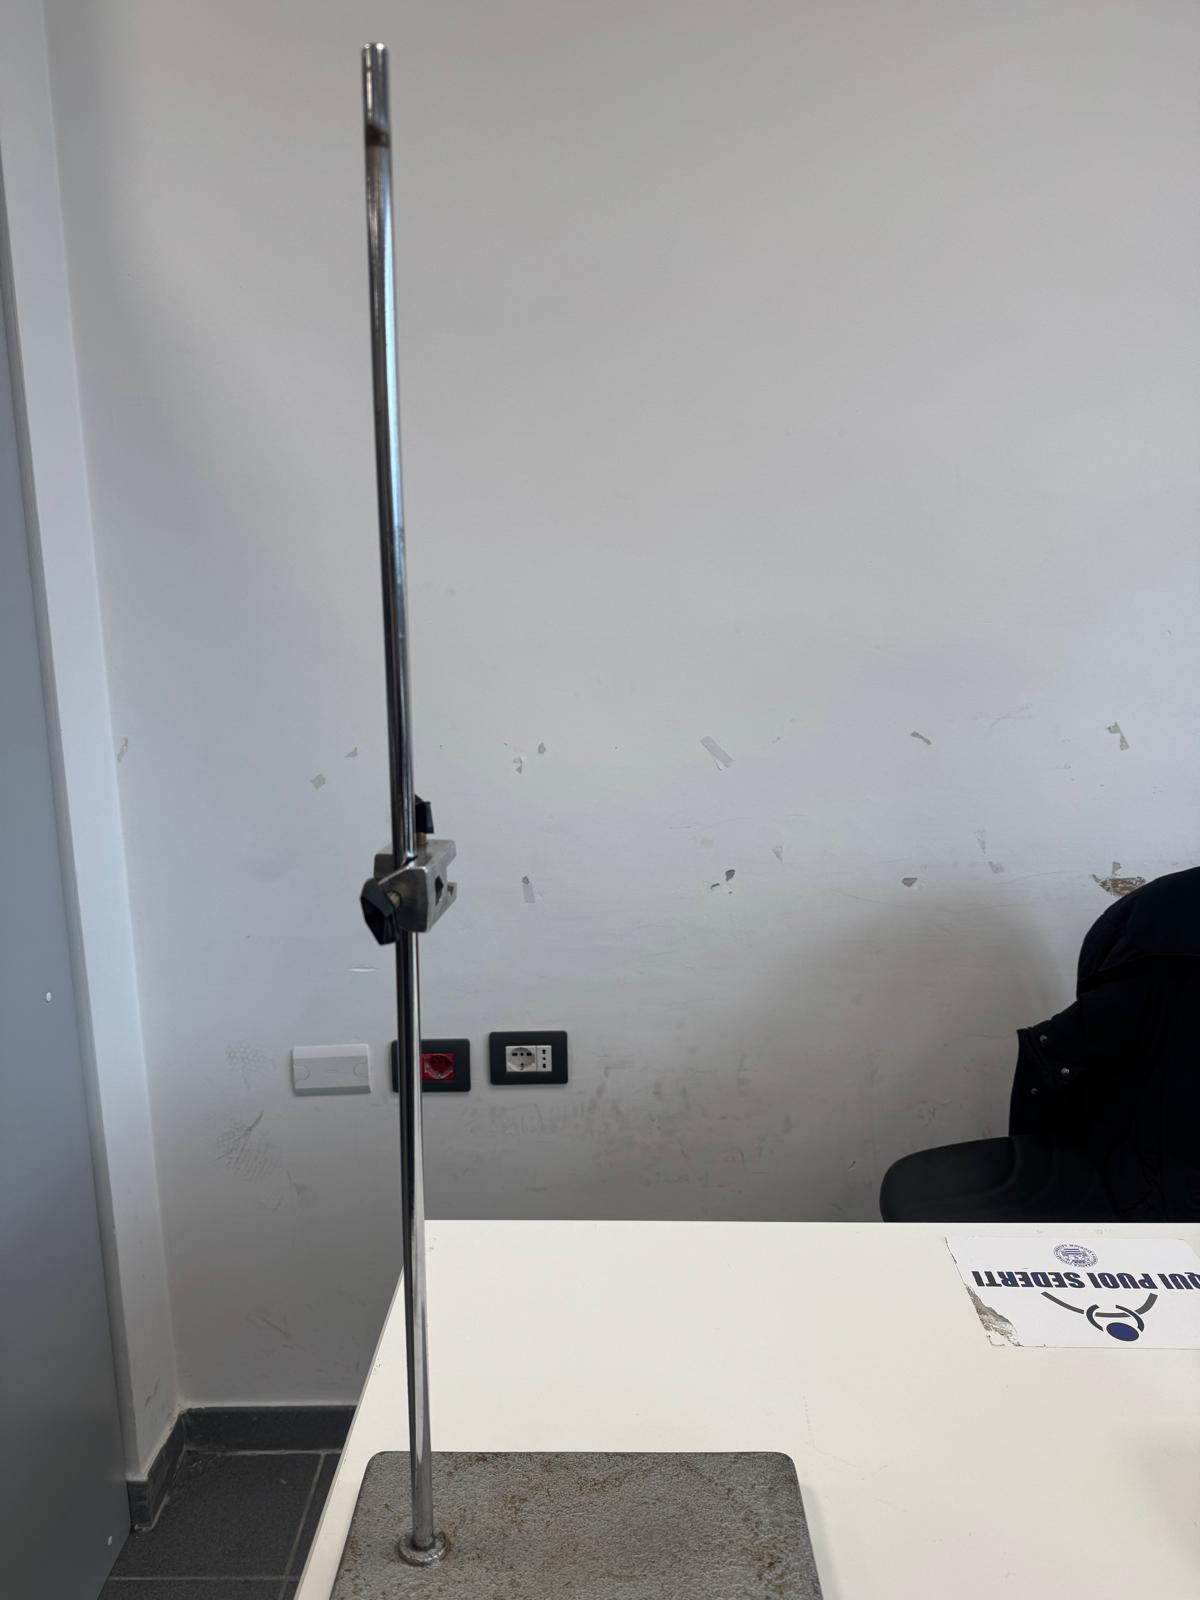
\includegraphics[width=0.65\textwidth]{./figures/asta}
	\caption{Asta assemblata utilizzata per l'esperimento. Si noti la differenza di altezza tra quest'ultima e la vaschetta.}
\end{figure}